\chapter{Label inference}
\section{Problem Statement}\label{\positionnumber}
A lot of data contains implicit patterns and structures~\cite{mitchell2006discipline}~\cite{carlsson2009topology} that is not reflected explicitly by the data model. Extracting those pieces of knowledge is the task of knowledge discovery and data mining~\cite{SIGKDD-2019-12-11}. \\

Nobel Laureate and ACM Turing award winner Herbert A. Simon wrote in his book "The Sciences of the Artificial": "Thus my central theme is that complexity frequently takes the form of hierarchy and that hierarchic systems have some common properties independent of their specific content. Hierarchy, I shall argue, is one of the central structural schemes that the architect of complexity uses."~\cite{simon2019sciences}.

Type taxonomies have been used in Object-Oriented programming to visualize inheritance and type hierarchies in Russell's Principia Mathematica to define a type system~\cite{whitehead1912principia, TUPPER2011369}.

When focusing on data objects or nodes in terms of the property graph model there is often an implicit hierarchy or taxonomy of types. Such an implicit type taxonomy may provide further insights about data as it may e.g. help in estimating cardinalities during query optimization, when keeping further statistics about the latent class distribution and may also reveal additional information about the type of instances, like how to categorize an instance, is it rare or special from a certain point view, is it an outlier, $\dots$. \\

For example in the yelp data set, the businesses may be further categorized in e.g. restaurants, spas, shopping malls, etc. One may further subdivide the restaurants by additional properties and features like cooking style (Italian, Asian, burgers, $\dots$) or  by location (Italian restaurants in New York, Asian restaurants in Manhattan).\\

The below example is motivated by the yelp data set. In the yelp data set instances are assigned categories by users of the yelp system. Inspecting them shows frequently category label distributions like in Tab. \ref{tab:running_ex}: \\
\begin{table}[htp]
     \centering
     \begin{tabular}{c c} \toprule
            Node.name & Node.labels \\ \midrule
            Fernando's & restaurant, Italian \\ 
            Arche & restaurant, Vietnamese \\ 
            Zum Elefanten & restaurant, Thai \\ 
            Campus Cafe & cafe, WiFi \\ 
            Endlicht & cafe, late-night \\ 
            Pano & cafe, breakfast \\
            Lago & shopping, mall \\ 
            Seerhein Center & shopping, cheap \\ 
            Seepark & Shopping, expensive \\ \bottomrule
        \end{tabular}
    \caption{A fictive example of business and user-defined associated labels.}
    \label{tab:running_ex}
\end{table}{}
Which may be visualized as taxonomy like in fig. \ref{fig:ex_hier}. \\
\fig{img/ex_hierarchy}{ex_hier}{The taxonomy that is implicit in the labels of the example in tab.\ref{tab:running_ex}}{1} \\
 In practice the categories are just informal strings, there is no notion of this structure in the current representation of the property graph model. In order to leverage this implicit taxonomy it needs to be made explicit. \\
 
Given a property graph model-based database, how can one extract such a taxonomy?
Finding classes or in other terms subsets of the input is what is addressed by clustering methods. Extracting a hierarchy of classes is what Hierarchical clustering copes with (see \fullref{3.1}). \\
In order to infer a hierarchy classes for nodes from a property graph model-based database, one may take various information into account: 
\begin{itemize}
    \item the user-defined labels only
    \item the properties of the node
    \item per node structural features of the underlying graph
    \item the properties of the relationships
    \item further constructed features based on previous steps
\end{itemize}
As briefly mentioned in chapter 2, different algorithms yield different clusterings as well as the same clustering algorithm with different features and parameters yields different clusterings. Thus in order to find a suitable taxonomy extraction method for the property graph model the following steps are subsequently performed:
\begin{enumerate}
    \item Find a suitable clustering algorithm that produces a taxonomy using a minimal feature set and different parameters to cover the space of algorithms and parameters as extensively as feasible.
    \item Find a suitable feature vector that also leverages the graph structure
\end{enumerate}
Each step has it's own requirements and objectives that are addressed in the subsequent sections, but both follow the same pipeline depicted in fig. \ref{fig:pipeline}. \\
\fig{img/pipeline.png}{pipeline}{The pipeline that is used to generate the taxonomy.}{1}


\section{Phase I: Algorithm Selection}\label{\positionnumber}
\subsection{Overview}\label{\positionnumber}
    In order to evaluate a wide range of algorithms, the pipeline uses the interface for clustering algorithms specified in \fullref{3}, that is adapted to the specific algorithm as necessary. \\
    During the algorithm selection stage, no data base is used and no graph structure is considered. Thus the data loading stage consists of reading data from a file in a certain format e.g. JSON.

\subsection{Data Generation: A Synthetic Data Set}\label{\positionnumber}
%% TODO: Pseudo code
The example given in \fullref{4.1} is inspired by the yelp data set and a synthetic one, that constructs label sets yielding a homogeneous taxonomy with a user-defined height and width when extracting the taxonomy by hand. The height is the number of levels in the hierarchy and the width is the number of children each inner node has. This allows to measure the extracted hierarchy against a simple ground truth. \\
Data sets are by nature incomplete \& noisy due to measurements or human errors.
So the data generator shall also be able to introduce noise, i.e. to add, remove or alter labels in the label set of an object in order to measure the robustness of the taxonomy extraction method. 
An example of the generated data is shown in table \ref{tab:datagen}.
\begin{table}[htp]
     \centering
     \begin{tabular}{c c} \toprule
            Node.name & Node.labels \\ \midrule
            0 & l0, l00 \\ 
            1 & l0, l01 \\ 
            2 & l0, l02 \\ 
            3 & l1, l10 \\ 
            4 & l1, l11 \\ 
            5 & l1, l12 \\
            6 & l2, l20 \\ 
            7 & l2, l21 \\ 
            8 & l2, l22 \\ \bottomrule
        \end{tabular}
    \caption{A sample of generated data for parameters height = 2, width = 3 and noise = 0 }
    \label{tab:datagen}
\end{table}{}

\subsection{Pre-Processing}\label{\positionnumber}
\subsubsection{Encoding Sets of Labels as Vectors}
\begin{algorithm}[htp]
    \KwIn{Set of Objects $O$, set of sets of Attributes $A = \{A_{o_0}, A_{o_1}, \dots \}$}
    \Parameters{No Parameters}
    \KwOut{A matrix $M$ of shape $|O| \times |A|$ with $m_{o,a} \in \{0, 1\}$} 
    \Begin{
        $M \rightarrow zeros(|O|, |A|)$\;
        \For{Object o in O} {
            \For{Attribute a in A}{
                \If{$a \in A_o$}{
                    $M[o,a] = 1$\;
                }
            }
        }
    }
\caption{Vectorize Labels}\label{vect}
\end{algorithm} 
After loading the data it needs to be converted into a representation that the clustering algorithms work on. Most clustering algorithms take a feature vector as input, that is a matrix of reals on some metric space. Character strings need to be transformed to comply with this requirement. Text Vectorization, also referred to as One-Hot encoding builds a matrix representation, given a set of string attributes per object.

Consider the example given in tab. \ref{tab:running_ex}. The vectorized representation of the example in tab. \ref{tab:running_ex} is given in tab. \ref{tab:vect_running_ex}
\begin{table}[htp]
     \centering
     \begin{tabular}{|c|c|c|c|c|c|c|c|c|c|c|c|c|} \hline
            Node.name & rest & ital & viet & thai & cafe & wifi & late & brea & shop & mall & chea & expe \\ \hline \hline
            Fernando's      & 1 & 1 & 0 & 0 & 0 & 0 & 0 & 0 & 0 & 0 & 0 & 0  \\  \hline
            Arche           & 1 & 0 & 1 & 0 & 0 & 0 & 0 & 0 & 0 & 0 & 0 & 0  \\  \hline
            ZumElefanten    & 1 & 0 & 0 & 1 & 0 & 0 & 0 & 0 & 0 & 0 & 0 & 0  \\ \hline
            CampusCafe      & 0 & 0 & 0 & 0 & 1 & 1 & 0 & 0 & 0 & 0 & 0 & 0 \\ \hline
            Endlicht        & 0 & 0 & 0 & 0 & 1 & 0 & 1 & 0 & 0 & 0 & 0 & 0 \\ \hline
            Pano            & 0 & 0 & 0 & 0 & 1 & 0 & 0 & 1 & 0 & 0 & 0 & 0 \\ \hline
            Lago            & 0 & 0 & 0 & 0 & 0 & 0 & 0 & 0 & 1 & 1 & 0 & 0 \\ \hline
            Seerhein Center & 0 & 0 & 0 & 0 & 0 & 0 & 0 & 0 & 1 & 0 & 1 & 0 \\ \hline
            Seepark         & 0 & 0 & 0 & 0 & 0 & 0 & 0 & 0 & 1 & 0 & 0 & 1\\ \hline
        \end{tabular}
    \caption{A vector representation of the example from tab. \ref{tab:running_ex} corresponding to $I$}
    \label{tab:vect_running_ex}
\end{table}{} \\


\subsection{Clustering}\label{\positionnumber}
\subsubsection{Compute Distance Matrix}\label{\positionnumber}
Some algorithms need the distance matrix as an input to the algorithm. To avoid computing the matirx multiple times it is precomputed once and reused if applicable. \\
Given that we cluster sets of labels, a suitable distance is the Jacquard distance, that is a similarity measure for sets~\cite{DBLP:journals/corr/Kosub16} and is symmetric. \\
\[\text{Jaccard Distance} d_J(A, B) = \frac{|A \cup B| - |A \cap B|}{|A \cup B|} \]
\begin{algorithm}[htp]
    \KwIn{A set of objects $O$}
    \Parameters{None}
    \KwOut{The pairwise distance matrix} 
    \Begin{
        matrix $\leftarrow$ nan($|O|$, $|O|$)\;
        \For{$o_i \in O$}{
            \For{$o_j \in O$}{
                \If{matrix[i][j] is NaN}{
                    matrix[i][j] = $d_J$($o_i$, $o_j$)\;
                    matrix[j][i] = matrix[i][j]\;
                }
            }
        }
        \Return matrix
    }
\caption{Pairwise Jaccard distance matrix}\label{distM}
\end{algorithm}

\subsubsection{Apply Clustering}\label{\positionnumber}
The methods described in \fullref{3.1.1}, \fullref{3.1.2}, \fullref{3.3.3} and \fullref{3.4.1} already produce hierarchies as outputs, so those methods may be applied to the pre-processed data without further clustering steps. All other approaches produce only "flat" clusters. Similarly to HDBSCAN, one can apply hierarchical clustering to overcome weaknesses of both approaches: Hierarchical Clustering is less computationally expensive when it is applied to a subset of the input that was clustered before with a more efficient clustering method. In order to do this, we first apply a non-hierarchical algorithm to the input data set. Then for each cluster take the intersection of the set of labels of all objects in the cluster in order to obtain a class description for all clusters. On those newly formed objects perform hierarchical clustering to generate a hierarchy. This comes with the obvious cost of loss of information, and is especially difficult noisy when data is noisy. Problems and ways to overcome those are discussed in \fullref{5}. \\
Further many clustering algorithms have parameters that need to be optimized for the data set, e.g. for k-Means the number of clusters needs to be known in advance.


\subsection{Post-Processing: Taxonomy Extraction}\label{\positionnumber}
Both approaches return A hierarchically ordered set of subsets of $O$ but with only one merge per tree depth level: This is a characteristic trait of a dendrogram and the most significant difference to other trees and tree-like structures. Instead of consisting of only $\log_k n$ levels it consists of $n$ levels. Thus the dendrogram can be flattened to get the corresponding "well-formed" tree of clusters - a taxonomy. \\
The output of agglomerative clustering is a linkage matrix, a matrix of shape $3 \times |merges|$, where column 0 contains the first merged cluster, column 1 the second merged cluster and column 2 the distance of the merged clusters, representing the hierarchically ordered set of subsets.
What the flattening intuitively does is aggregating merges where clusters have been merged consecutively and with the same distance. \\
For instance $C_{00} = C_0 \cup C_1$ with distance $d$, $C_{01} = C_{00} \cup C_2$ with distance $d$, and $C_{02} = C_{01} \cup C_3$ with distance $d$ would be aggregated into $C_{00} = C_0 \cup C_1 \cup C_2, \cup C_3$ with distance $d$. 
\begin{algorithm}[htp]
    \KwIn{linkage matrix $lM$}
    \Parameters{None}
    \KwOut{A taxonomy of $O$} 
    \Begin{
        previousRow $\leftarrow [-1, -1, -1]$\;
        taxonomy $\leftarrow$ new Map\;
        cluster $\leftarrow$ new Set\;
        distance $\leftarrow$ -1\;
        consecutive = False\;
        \For{row in $lM$}{
            \If{(row[0] == previousRow[0] or row[1] == previousRow[1])  and row[2] == previousRow[2]}{
                \If{taxonomy is not empty and not consecutive}{
                    taxonomy.removeLast()\;
                    cluster.add(previousRow[0], previousRow[1])\;
                }
                 distance $\leftarrow$ row[2]\;
                 cluster.add(row[0], row[1])\;
                 consecutive $\leftarrow$ True\;
            }{
                \If{consecutive}{
                    taxonomy.add(clusters, distance)\;
                    cluster.clear()\;
                    distance = -1\;
                }
                consecutive = False\;
                taxonomy.add(\{row[0], row[1]\}, row[2])
            }
        }
        return cluster
    }
\caption{Taxonomy Extraction from a Dendrogram}\label{taxo}
\end{algorithm}

\begin{figure}[htp]
    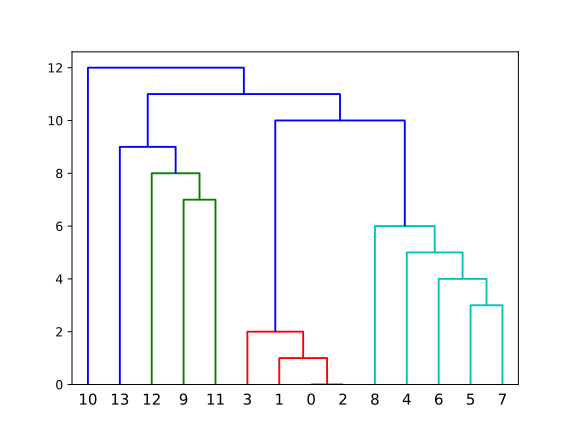
\includegraphics[width=0.49\textwidth]{img/extract_ex_dendro.png}
        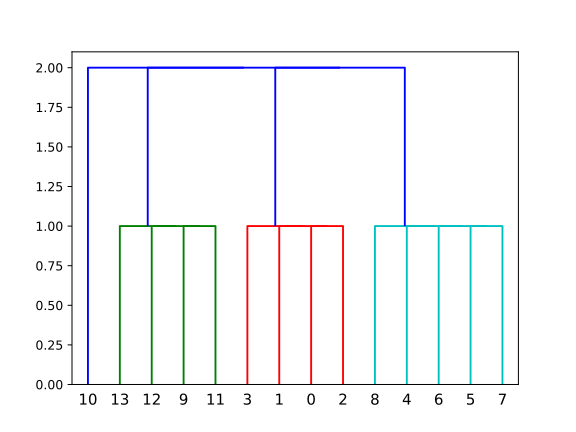
\includegraphics[width=0.49\textwidth]{img/extract_ex_taxo.png}
    \caption{The Input and output of the taxonomy extraction heuristic}
    \label{fig:my_label}
\end{figure} 
 
 \subsection{Evaluation \& Visualization}\label{\positionnumber}
 In order to evaluate the so extracted taxonomy, a way of measuring the deviation from the ground truth is needed. The Tree Edit Distance is a measure defined as the minimum cost sequence of edit operations to a tree $T$ to transform it to another tree $T'$~\cite{Tai:1979:TCP:322139.322143}. A computationally more efficient and less memory consuming implementation is APTED by Pawlik et al~\cite{pawlik2016tree}, which is used for evaluation. The visualization provides illustrations of the dendrogram, the taxonomy, the flat clusters and the resulting tree edit distance.

\section{Phase 2: Graph-aware Taxonomy Inference}\label{\positionnumber}
In the second phase the clustering algorithm is fixed to Cobweb as 
\begin{itemize}
    \item it's able to deal with all kinds of values without pre-processing, even missing values and faulty values
    \item it's hierarchical, producing not a dendrogram but rather a data driven hierarchy of variable branching factor, that is no post-processing is needed
    \item regarding Cobweb, the limiting factor is not memory, i.e. it's potentially more scalable to very large data sets
    \item it has a probabilistic (i.e. easily interpretable as fuzzy) concept description, i.e. there is no need for a fuzzy intersection or any other intermediate steps and it provides additional statistics regarding the values and their support in the data set
    \item Cobweb does not have additional parameters that need to be optimized
\end{itemize}
However note that any of the other approaches can also be used. Some of the practical problems that are discussed in the next chapter may easily be solved, so the following is a general purpose strategy for clustering in graph context, leveraging the underlying structure in the graph as well as object descriptions given by attribute value pairs.
Pre-processing and clustering is combined in this approach, as feature extraction is generally considered as a pre-processing step~\cite{han2011data}, but the feature-extraction already involves clustering. \\
The first step of the pre-processing/clustering phase \fullref{4.3.3.1} elaborates on the extraction of purely attribute value-based features and takes a rather object-oriented view on the problem of clustering in the property graph model, but is also applicable on non-graph structures. Instead of clustering nodes and edges, apply the technique to all different kinds of objects in the problem context, to obtain those features. 
The second step focuses on structural features to be extracted from the data base. The third step considers the final clustering step.


\subsection{Data Generation: The LDBC SNB Benchmark}
\fig{img/ldbc_snb.png}{ldbc}{The schema for the LDBC SNB benchmark}{0.5}
The Linked Data Benchmark Council (LDBC) consists of a group of industrial and academic organizations that research on data bases e.g. the Technische Universitaet Muenchen, Neo4J or the Vrije Universiteit Amsterdam. The LDBC social network benchmark aims at providing the following to the users:
\begin{itemize}
    \item Cover most demands that arise when managing data
    \item Modular structured, i.e. may be broken into pieces without large overhead
    \item Balanced selection of challenges
    \item Modest implementation cost
    \item Reproducibility and documentation
\end{itemize}
The synthetic data set that is generateable using the software provided by the LDBC mimics a social network that follows the schema in fig. \ref{fig:ldbc}. To ensure realism the authors modeled data link distributions as found in real world social networks like Facebook and provided attribzte values found in DBpedia. They also pay attention to regularities like homophily in the links of social networks, i.e. in a social context there tend to be more connections between people that behave similar and have similar interests. To ensure scalability of the generation process, it is implemented using the MapReduce paradigm.

\subsection{Data Loading: Neo4J Data Set Import}
Loading a data set in Neo4J requires adding it to the data base. As each data set shall reside in an own data base, each needs to be imported in an own instance of Neo4J, either using a query or an import tool. When the import has finished, all nodes and edges are traversable in Neo4J and certain statistics e.g. the node degree are available for querying from within the system. 

\subsection{Pre-Processing \& Clustering}
\subsubsection{Generalizing Node and Relationship Instances}\label{\positionnumber}
In order to discover sub-types and possible generalizations, the goal of the first step is to group all kinds of classes in an own Cobweb tree. Having an own tree for each kind is not required but reduces negative effects of ordering. There are extensions to the Cobweb framework to reduce ordering effects after insertion, that may be considered for future work. \\
In the property graph model that is one Cobweb tree for the nodes and one for the edges. What each of these trees captures are all possible node and edge sub-types present in the data set, grouped by properties and labels for nodes or relationship type for edges. Essentially the output then represents the underlying distribution of attribute value pairs. That is combining all information of the so constructed trees should be sufficient to generate a new data set that has similar objects compared to the one used for extraction, i.e. the distribution of object descriptions is partitioned and  learned. \\
In order to generalize one can set a cutoff level and replace the properties of the current node or relationship with the concept label at the chosen level. For instance when looking at road network nodes (crossings) which have no properties and edges (roads) where all roads have the same type and possibly distinct distances (e.g. 1 Km or 50 Km) the output of the procedure would optimally yield partitions based on the road length. Adding more properties like the road width would then yield sub-types like long and wide, short and tight etc. From an intuitive point of view this makes a lot of sense as humans also categorize roads by their attributes (e.g. a long and wide street is very likely a motor way, a long and medium wide street is a country road, a short and tight road is in a rather residential area, a short and wide road is probably a major city road and so on). \\
We want to infer labels, i.e. features for nodes, so why clustering and generalizing relationships? When generalizing relationships similar ones aggregate in type, so a node that has a lot of conceptually different ones may be differentiated by a node that has only relationships of one conceptual type. \\
egoDegPerType

\subsubsection{Extracting Structural Features}\label{\positionnumber}
As we focus on a label hierarchy we want to extract structural features from the nodes (compare with \fullref{2.1}: Nodes have labels, relationships have a type).
When no properties are present at all then strucutral features are the information that can be extracted. Following the approach of Henderson et al. and Neumann et al. described in \fullref{3.5} the features that are extracted are
\begin{itemize}
    \item the degree of the node
    \item the average neighbour degree
    \item the degree per relationship type of the node (also capturing the characteristic set)
    \item the average degree per relationship type of the neighbours (also capturing the average characteristic set of the neighbours)
    \item The amount of relationships that are outgoing from the ego net
    \item the amount of relationships that are incomming to the egonet
\end{itemize}
As the proposed method shall be a proof of concepts, the extracted features are neither complete nor exhaustive. Additionally weighted, directed and recursively aggregated versions of the above should also be considered.

\subsubsection{Clustering the Feature Vector}
Adding all so extracted features together produces a summary of the node that contains the following information:
\begin{itemize}
    \item Node property concept label
    \item Aggregated relationship property concepts
    \item structural features
\end{itemize}
Note that more semantic or concept-based features can be extracted, like aggregated neighbour property concepts or regarding relationships what node property types are connected by a certain edge concept. 
Applying Cobweb to those feature vector yields something similar to Henderson's role extraction~\cite{henderson2012rolx}, but with additional information: Not only the role is analyzed but also the characteristics of the object itself. What is captured as concepts in the hierarchy or taxonomy constructed by Cobweb is how a node generally looks like, that is the distribution over the properties a node has, the relation a node has and of what type the relations are. \\
Returning to the road network example this would classify the crossings by the street types and their properties, meaning that a motor way junction (a few wide long streets crossing) should end up in a different concept than a country road crossing (a few long but not too wide streets crossing). This is of course dependent on the cutoff level chosen. \\
From a theoretical point of view the proposed method is able to deal with object-oriented data, triplets like in RDF and a mixture of both models, that is the property graph model. It's able to summarize information and extract probabilistic concepts from relations, components and thereof constructed objects and graphs in a parameter-free and unsupervised manner. 


\subsection{Evaluation \& Visualization}
Again, the Tree Edit Distance and the APTED implementation is used to compare the extracted concepts to the ground truth. In this case the ground truth is the LDBC SNB schema as defined in the specification. The visualization


\section{Implementation}
\subsection{Phase 1}
% TODO quote sklearn, pyclustering, trestle
The implementation of phase 1 uses Python 3, SciKit-learn and PyClustering as basis. Overall 16 different algorithms have been tried, where only 4 of them are described in this thesis for the sake of brevity. During the implementation and experimentation the author found a bug in SciKit-learn and fixed it. As most of the algorithms require parameters a parameter optimization technique was applied namely Grid Search. In order to use the Grid Search whichs implementation is in sklearn with PyClustering, a wrapper around the algorithms of the latter was implemented. For conceptual clustering the TRESTLE algorithm from the concept formation package was used.


\subsection{Phase 2}
% TODO cite cypher
In order to implement the proposed method using Neo4J and potentially move it to a deeper level in the architecture of the data base it was implemented as a Cypher procedure that can be called from the query language. The implementation of Cobweb was done by the author from scratch as well as all feature extraction traversals of the graph, besides the node degree. For testing purposes, a annotation-based data base setup and import framework was written, provided by Manuel Hotz and refine by the author. \\
In order to boost the computational performance a multi-threaded version was implemented but yielded high contention that cancelled the concurrency gains in Cobweb. Clustering nodes and edges and extracting structual features concurrently resulted in a noticable performance gain. There is further space for optimization regarding memory access patterns, caching and storing intermediate values to avoid the computation of the same value over and over again. A more comprehensive discussion of the improvals to the method itself and the run time can be found in \fullref{6}. \\
